% Options for packages loaded elsewhere
\PassOptionsToPackage{unicode}{hyperref}
\PassOptionsToPackage{hyphens}{url}
%
\documentclass[
]{article}
\author{}
\date{\vspace{-2.5em}}

\usepackage{amsmath,amssymb}
\usepackage{lmodern}
\usepackage{iftex}
\ifPDFTeX
  \usepackage[T1]{fontenc}
  \usepackage[utf8]{inputenc}
  \usepackage{textcomp} % provide euro and other symbols
\else % if luatex or xetex
  \usepackage{unicode-math}
  \defaultfontfeatures{Scale=MatchLowercase}
  \defaultfontfeatures[\rmfamily]{Ligatures=TeX,Scale=1}
\fi
% Use upquote if available, for straight quotes in verbatim environments
\IfFileExists{upquote.sty}{\usepackage{upquote}}{}
\IfFileExists{microtype.sty}{% use microtype if available
  \usepackage[]{microtype}
  \UseMicrotypeSet[protrusion]{basicmath} % disable protrusion for tt fonts
}{}
\makeatletter
\@ifundefined{KOMAClassName}{% if non-KOMA class
  \IfFileExists{parskip.sty}{%
    \usepackage{parskip}
  }{% else
    \setlength{\parindent}{0pt}
    \setlength{\parskip}{6pt plus 2pt minus 1pt}}
}{% if KOMA class
  \KOMAoptions{parskip=half}}
\makeatother
\usepackage{xcolor}
\IfFileExists{xurl.sty}{\usepackage{xurl}}{} % add URL line breaks if available
\IfFileExists{bookmark.sty}{\usepackage{bookmark}}{\usepackage{hyperref}}
\hypersetup{
  hidelinks,
  pdfcreator={LaTeX via pandoc}}
\urlstyle{same} % disable monospaced font for URLs
\usepackage[margin=1in]{geometry}
\usepackage{color}
\usepackage{fancyvrb}
\newcommand{\VerbBar}{|}
\newcommand{\VERB}{\Verb[commandchars=\\\{\}]}
\DefineVerbatimEnvironment{Highlighting}{Verbatim}{commandchars=\\\{\}}
% Add ',fontsize=\small' for more characters per line
\usepackage{framed}
\definecolor{shadecolor}{RGB}{248,248,248}
\newenvironment{Shaded}{\begin{snugshade}}{\end{snugshade}}
\newcommand{\AlertTok}[1]{\textcolor[rgb]{0.94,0.16,0.16}{#1}}
\newcommand{\AnnotationTok}[1]{\textcolor[rgb]{0.56,0.35,0.01}{\textbf{\textit{#1}}}}
\newcommand{\AttributeTok}[1]{\textcolor[rgb]{0.77,0.63,0.00}{#1}}
\newcommand{\BaseNTok}[1]{\textcolor[rgb]{0.00,0.00,0.81}{#1}}
\newcommand{\BuiltInTok}[1]{#1}
\newcommand{\CharTok}[1]{\textcolor[rgb]{0.31,0.60,0.02}{#1}}
\newcommand{\CommentTok}[1]{\textcolor[rgb]{0.56,0.35,0.01}{\textit{#1}}}
\newcommand{\CommentVarTok}[1]{\textcolor[rgb]{0.56,0.35,0.01}{\textbf{\textit{#1}}}}
\newcommand{\ConstantTok}[1]{\textcolor[rgb]{0.00,0.00,0.00}{#1}}
\newcommand{\ControlFlowTok}[1]{\textcolor[rgb]{0.13,0.29,0.53}{\textbf{#1}}}
\newcommand{\DataTypeTok}[1]{\textcolor[rgb]{0.13,0.29,0.53}{#1}}
\newcommand{\DecValTok}[1]{\textcolor[rgb]{0.00,0.00,0.81}{#1}}
\newcommand{\DocumentationTok}[1]{\textcolor[rgb]{0.56,0.35,0.01}{\textbf{\textit{#1}}}}
\newcommand{\ErrorTok}[1]{\textcolor[rgb]{0.64,0.00,0.00}{\textbf{#1}}}
\newcommand{\ExtensionTok}[1]{#1}
\newcommand{\FloatTok}[1]{\textcolor[rgb]{0.00,0.00,0.81}{#1}}
\newcommand{\FunctionTok}[1]{\textcolor[rgb]{0.00,0.00,0.00}{#1}}
\newcommand{\ImportTok}[1]{#1}
\newcommand{\InformationTok}[1]{\textcolor[rgb]{0.56,0.35,0.01}{\textbf{\textit{#1}}}}
\newcommand{\KeywordTok}[1]{\textcolor[rgb]{0.13,0.29,0.53}{\textbf{#1}}}
\newcommand{\NormalTok}[1]{#1}
\newcommand{\OperatorTok}[1]{\textcolor[rgb]{0.81,0.36,0.00}{\textbf{#1}}}
\newcommand{\OtherTok}[1]{\textcolor[rgb]{0.56,0.35,0.01}{#1}}
\newcommand{\PreprocessorTok}[1]{\textcolor[rgb]{0.56,0.35,0.01}{\textit{#1}}}
\newcommand{\RegionMarkerTok}[1]{#1}
\newcommand{\SpecialCharTok}[1]{\textcolor[rgb]{0.00,0.00,0.00}{#1}}
\newcommand{\SpecialStringTok}[1]{\textcolor[rgb]{0.31,0.60,0.02}{#1}}
\newcommand{\StringTok}[1]{\textcolor[rgb]{0.31,0.60,0.02}{#1}}
\newcommand{\VariableTok}[1]{\textcolor[rgb]{0.00,0.00,0.00}{#1}}
\newcommand{\VerbatimStringTok}[1]{\textcolor[rgb]{0.31,0.60,0.02}{#1}}
\newcommand{\WarningTok}[1]{\textcolor[rgb]{0.56,0.35,0.01}{\textbf{\textit{#1}}}}
\usepackage{graphicx}
\makeatletter
\def\maxwidth{\ifdim\Gin@nat@width>\linewidth\linewidth\else\Gin@nat@width\fi}
\def\maxheight{\ifdim\Gin@nat@height>\textheight\textheight\else\Gin@nat@height\fi}
\makeatother
% Scale images if necessary, so that they will not overflow the page
% margins by default, and it is still possible to overwrite the defaults
% using explicit options in \includegraphics[width, height, ...]{}
\setkeys{Gin}{width=\maxwidth,height=\maxheight,keepaspectratio}
% Set default figure placement to htbp
\makeatletter
\def\fps@figure{htbp}
\makeatother
\setlength{\emergencystretch}{3em} % prevent overfull lines
\providecommand{\tightlist}{%
  \setlength{\itemsep}{0pt}\setlength{\parskip}{0pt}}
\setcounter{secnumdepth}{-\maxdimen} % remove section numbering
\usepackage{hyperref}
\usepackage{amsmath}
\usepackage{amssymb}
\usepackage{graphicx}
\usepackage{fontspec}
\usepackage{xcolor}
\usepackage{tikz}
\definecolor{green}{RGB}{0, 100, 0}
\setmainfont{Times New Roman}
\setsansfont{Times New Roman}
\setmonofont{Courier New}
\usepackage[margin=1in]{geometry}
\usepackage{titlesec}
\titleformat{\section}{\Huge\bfseries\color{green}}{\thesection}{1em}{}
\titleformat{\subsection}{\huge\bfseries\color{green}}{\thesubsection}{1em}{}
\titleformat{\subsubsection}{\LARGE\bfseries\color{green}}{\thesubsubsection}{1em}{}
\usepackage{tocloft}
\renewcommand{\cftsecfont}{\small}
\renewcommand{\cftsubsecfont}{\footnotesize}
\renewcommand{\cftsecpagefont}{\small}
\renewcommand{\cftsubsecpagefont}{\footnotesize}
\renewcommand{\cftsecleader}{\cftdotfill{\cftdotsep}}
\ifLuaTeX
  \usepackage{selnolig}  % disable illegal ligatures
\fi

\begin{document}

\begin{titlepage}
    \begin{center}
    % Début de la bordure avec TikZ
    \begin{tikzpicture}[remember picture, overlay] % overlay = force TikZ à dessiner par-dessus le contenu existant de la page, plutôt que de réserver un espace supplémentaire pour le dessin, remember = lorsque vous voulez dessiner par rapport à la position exacte de la page
    
    % Dessiner la bordure verte
    \draw[
        line width=5pt, 
        green, 
        rounded corners=15pt
    ] 
        ([xshift=10pt, yshift=-10pt]current page.north west) rectangle
        ([xshift=-10pt, yshift=10pt]current page.south east);
    
    % Dessiner la bordure jaune
    \draw[
        line width=5pt, 
        yellow, 
        rounded corners=15pt
    ] 
        ([xshift=15pt, yshift=-15pt]current page.north west) rectangle
        ([xshift=-15pt, yshift=15pt]current page.south east);
    
    % Dessiner la bordure rouge
    \draw[
        line width=5pt, 
        red, 
        rounded corners=15pt
    ] 
        ([xshift=20pt, yshift=-20pt]current page.north west) rectangle
        ([xshift=-20pt, yshift=20pt]current page.south east);
    
    \end{tikzpicture}
        
\includegraphics[width=7cm]{../Figures/LOGO1.jpeg} \\[0.1cm]  % 
        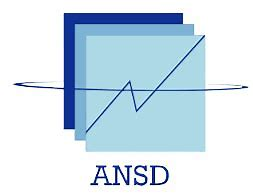
\includegraphics[width=6cm]{../Figures/LOGO2.jpeg} \\[0.1cm] % 
        
        \textbf{\large Agence nationale de la Statistique et de la Démographie (ANSD)}\\[0.2cm]
        
        
\includegraphics[width=4cm]{../Figures/LOGO3.jpeg} \\[0.1cm]  % 
        
        \textbf{\large Ecole nationale de la Statistique et de l'Analyse économique Pierre Ndiaye (ENSAE)}\\[0.4cm]
        
        \textit{\LARGE Semestre 2 :Projet statistique avec R }\\[0.3cm]
        \textit{\LARGE  }\\[0.3cm]

        \textbf{\Huge \color{green} \textsf{TP 5 : MERGING}}\\[0.2cm]
        
        \begin{minipage}{0.5\textwidth}
    \begin{flushleft} \large
        \emph{\textsf{Rédigé par :}}\\
        \textbf{Alioune Abdou Salam Kane}\\
        \textbf{Khadidiatou Diakhaté}\\
        \textbf{Ange Emilson Rayan Rahérinasolo}\\
        \textbf{Awa Diaw}\\
        \textit{Elèves en ISE 1 cycle long}
    \end{flushleft}
\end{minipage}
        \hfill
        \begin{minipage}{0.4\textwidth}
            \begin{flushright} \large
                \emph{\textsf{Sous la supervision de :}} \\
                \textbf{M. Aboubacre HEMA}\\
                \textit{Research Analyst }
            \end{flushright}
        \end{minipage}

        \vfill 

        {\large \textsf{Année scolaire : 2024/2025}}\\[0.5cm]
        
    \end{center}
\end{titlepage}  

\hypertarget{sommaire}{%
\subsection{Sommaire}\label{sommaire}}

\begin{itemize}
\tightlist
\item
  \protect\hyperlink{introduction}{Introduction}
\item
  \protect\hyperlink{installations-nuxe9cessaires}{1. Installations
  nécessaires}
\item
  \protect\hyperlink{chargement-des-fichiers}{2. Chargement des
  fichiers}
\item
  \protect\hyperlink{duplication-de-la-var-commune-dans-la-base-ehcvm}{3.
  Duplication de la var commune dans la base EHCVM}
\item
  \protect\hyperlink{premiuxe8re-fusion}{4. Première fusion}
\item
  \protect\hyperlink{seconde-fusion}{5. Seconde fusion}
\item
  \protect\hyperlink{vuxe9rification}{6. Vérificatio}
\item
  \protect\hyperlink{sauvegarde}{7. Sauvegarde}
\item
  \protect\hyperlink{conclusion}{Conclusion}
\end{itemize}

\newpage

\hypertarget{introduction}{%
\section{Introduction}\label{introduction}}

Le projet \textbf{TP4 : MERGING} a pour objectif principal de préparer
un fichier enrichi en fusionnant les données provenant de deux sources
importantes : l'\textbf{Enquête Harmonisée sur les Conditions de Vie des
Ménages (EHCVM) 2021} et le \textbf{Humanitarian Data Exchange (HDX)}.
Le défi majeur de ce projet réside dans la gestion des différences de
format et de nomenclature des communes entre ces deux bases de données,
ce qui nécessite un processus minutieux de nettoyage et de préparation
des données.

Afin de mener à bien cette tâche, nous avons utilisé \textbf{Excel} pour
effectuer les premières étapes de traitement des données. Tout d'abord,
nous avons créé un troisième fichier vecteur à deux variables où chacune
servait de clé unique pour la fucion avec les 2 datasets initiaux.

Cette approche nous a évité d'altérer les variables de base, tout en
réduisant le risque d'erreurs humaines.Les filtres et les recherches ont
automatisé de nombreuses étapes fastidieuses, offrant ainsi un gain de
temps et d'efficacité dans le traitement des données. En outre, la
vérification approfondie des communes a été réalisée afin de valider
leur présence dans la base de référence \textbf{HDX}. Les communes mal
écrites (exceptés ceux représentées en nombre)ont été corrigées grace à
la 2e base. Pour celles manquantes dans le HDX mais présentes dans le
EHCVM 2021, une exploraton de cette dernière avec la variable ``chef
lieu'' a permis de confirmer ou modifier le nom de la commune.

Ci-dessous, les sept principales étapes réalisées dans le traitement des
données à l'aide de \textbf{R} pour obtenir notre base finale.

\hypertarget{installations-nuxe9cessaires}{%
\section{1. Installations
nécessaires}\label{installations-nuxe9cessaires}}

Dans ce projet, nous utilisons plusieurs packages essentiels pour
manipuler et analyser les données. Afin de garantir que chaque package
est installé uniquement si nécessaire, nous avons défini une fonction
\emph{install\_if\_missing}. Cette fonction vérifie si le package est
déjà installé, et dans le cas contraire, l'installe automatiquement.

Voici les packages installés et chargés pour ce projet : \emph{readr},
\emph{readxl}, et \emph{dplyr} (Data Plyr ou dplyr fait référence à un
package plus ancien \emph{plyr} pour la manipulation de données). Le
code ci-dessous s'assure que ces packages sont disponibles avant d'être
utilisés dans le traitement des données :

\begin{Shaded}
\begin{Highlighting}[]
\NormalTok{packages }\OtherTok{\textless{}{-}} \FunctionTok{c}\NormalTok{(}\StringTok{"readr"}\NormalTok{, }\StringTok{"readxl"}\NormalTok{, }\StringTok{"dplyr"}\NormalTok{)}
\NormalTok{install\_if\_missing }\OtherTok{\textless{}{-}} \ControlFlowTok{function}\NormalTok{(pkg) \{}
  \ControlFlowTok{if}\NormalTok{ (}\SpecialCharTok{!}\FunctionTok{requireNamespace}\NormalTok{(pkg, }\AttributeTok{quietly =} \ConstantTok{TRUE}\NormalTok{)) }\FunctionTok{install.packages}\NormalTok{(pkg)}
\NormalTok{\}}
\FunctionTok{invisible}\NormalTok{(}\FunctionTok{lapply}\NormalTok{(packages, install\_if\_missing))}

\CommentTok{\# Charger les packages}
\FunctionTok{library}\NormalTok{(readr)      }
\end{Highlighting}
\end{Shaded}

\begin{verbatim}
## Warning: le package 'readr' a été compilé avec la version R 4.4.2
\end{verbatim}

\begin{Shaded}
\begin{Highlighting}[]
\FunctionTok{library}\NormalTok{(readxl)  }
\FunctionTok{library}\NormalTok{(dplyr)}
\end{Highlighting}
\end{Shaded}

\begin{verbatim}
## 
## Attachement du package : 'dplyr'
\end{verbatim}

\begin{verbatim}
## Les objets suivants sont masqués depuis 'package:stats':
## 
##     filter, lag
\end{verbatim}

\begin{verbatim}
## Les objets suivants sont masqués depuis 'package:base':
## 
##     intersect, setdiff, setequal, union
\end{verbatim}

\hypertarget{chargement-des-fichiers}{%
\section{2. Chargement des fichiers}\label{chargement-des-fichiers}}

Les \textbf{chemins relatifs} ont été utilisés pour spécifier les
fichiers. L'avantage d'utiliser un chemin relatif plutôt qu'absolu
réside dans la portabilité du code, facilitant ainsi l'exécution du
script sur différentes machines sans avoir à modifier les chemins
d'accès. Cela garantit également que le code fonctionne indépendamment
de l'emplacement exact du projet sur l'ordinateur.

\begin{Shaded}
\begin{Highlighting}[]
\NormalTok{EHCVM\_data }\OtherTok{\textless{}{-}} \FunctionTok{read\_csv}\NormalTok{(}\StringTok{"../Data/ehcvm\_individu\_mli2021.csv"}\NormalTok{,}
                       \AttributeTok{show\_col\_types =} \ConstantTok{FALSE}\NormalTok{)  }
\end{Highlighting}
\end{Shaded}

\begin{verbatim}
## Warning: One or more parsing issues, call `problems()` on your data frame for details,
## e.g.:
##   dat <- vroom(...)
##   problems(dat)
\end{verbatim}

\begin{Shaded}
\begin{Highlighting}[]
\CommentTok{\# Certaines col ne sont pas bien reconnus }
\CommentTok{\#Certaines colonnes ne sont pas bien reconnues (Par exemple,}
\CommentTok{\#une colonne censée être numérique peut contenir des caractères}
\CommentTok{\#ou bien une colonne attendue comme texte (chr) est vide, ce qui}
\CommentTok{\#cause l\textquotesingle{}erreur). Comme cela n\textquotesingle{}affecte pas l\textquotesingle{}exécution, on masque }
\CommentTok{\#l\textquotesingle{}avis.}

\CommentTok{\#View(EHCVM\_data)}

\NormalTok{vecteur\_data }\OtherTok{\textless{}{-}} \FunctionTok{read\_excel}\NormalTok{(}\StringTok{"../Data/Groupe3\_tp4\_vecteur.xlsx"}\NormalTok{)   }

\CommentTok{\#View(vecteur\_data)}

\NormalTok{HDX\_data }\OtherTok{\textless{}{-}} \FunctionTok{read\_excel}\NormalTok{(}\StringTok{"../Data/mli\_adminboundaries\_tabulardata.xlsx"}\NormalTok{)}
\CommentTok{\#View(HDX\_data)}
\end{Highlighting}
\end{Shaded}

\hypertarget{duplication-de-la-var-commune-dans-la-base-ehcvm}{%
\section{3. Duplication de la var commune dans la base
EHCVM}\label{duplication-de-la-var-commune-dans-la-base-ehcvm}}

Pour effectuer des comparaisons avvec la base finale à générer, nous
avons dupliqué la colonne des communes.

\begin{Shaded}
\begin{Highlighting}[]
\CommentTok{\# Dupliquer la colonne commune dans EHCVM\_datapour conserver}
\CommentTok{\#les communes de EHCVM pour des comparaisons ultérieures}

\NormalTok{EHCVM\_data }\OtherTok{\textless{}{-}}\NormalTok{ EHCVM\_data }\SpecialCharTok{\%\textgreater{}\%}
  \FunctionTok{mutate}\NormalTok{(}\AttributeTok{Commune\_EHCVM\_dupli =} \StringTok{\textasciigrave{}}\AttributeTok{commune}\StringTok{\textasciigrave{}}\NormalTok{)}

\CommentTok{\#View(EHCVM\_data)}
\end{Highlighting}
\end{Shaded}

\hypertarget{premiuxe8re-fusion}{%
\section{4. Première fusion}\label{premiuxe8re-fusion}}

La première fusion est réalisée entre les données des individus issues
de l'EHCVM et le fichier vecteur contenant les informations
géographiques des communes. Pour ce faire, nous utilisons la fonction
left\_join du package dplyr, qui permet d'associer les deux jeux de
données sur la base de la variable \emph{Commune\_EHCVM\_dupli}
(présente dans EHCVM\_data) et \emph{Admin3\_EHCVM} (présente dans
vecteur\_data). Cette fusion est effectuée dans une relation
``many-to-many'', ce qui signifie qu'une commune peut apparaître
plusieurs fois dans chaque fichier, en fonction des individus qui y sont
associés.

\begin{Shaded}
\begin{Highlighting}[]
\CommentTok{\# Merge 1 : Individus + Fichier Vecteur}
\NormalTok{merge1 }\OtherTok{\textless{}{-}}\NormalTok{ EHCVM\_data }\SpecialCharTok{\%\textgreater{}\%}
  \FunctionTok{left\_join}\NormalTok{(vecteur\_data, }\AttributeTok{by =} \FunctionTok{c}\NormalTok{(}\StringTok{"Commune\_EHCVM\_dupli"} \OtherTok{=} \StringTok{"Admin3\_EHCVM"}\NormalTok{),}
            \AttributeTok{relationship =} \StringTok{"many{-}to{-}many"}\NormalTok{) }

\CommentTok{\#View (merge1)}
\end{Highlighting}
\end{Shaded}

\hypertarget{seconde-fusion}{%
\section{5. Seconde fusion}\label{seconde-fusion}}

La deuxième fusion consiste à combiner les résultats de la première
fusion avec la base HDX, qui contient des informations administratives
supplémentaires. Comme dans la première fusion, nous utilisons à nouveau
la fonction left\_join de dplyr pour lier les données sur la base de la
variable \emph{Admin3\_HDX} (dans le jeu de données merge1) et
\emph{admin3Name\_fr} (dans la base HDX).

Cette fusion permet d'intégrer les informations administratives de la
base HDX à notre jeu de données final, offrant ainsi une vue plus
complète des communes du Mali.

\begin{Shaded}
\begin{Highlighting}[]
\CommentTok{\# Merge 2 : Résultat précédents Base HDX}
\NormalTok{final\_data }\OtherTok{\textless{}{-}}\NormalTok{ merge1 }\SpecialCharTok{\%\textgreater{}\%}
  \FunctionTok{left\_join}\NormalTok{(HDX\_data, }\AttributeTok{by =} \FunctionTok{c}\NormalTok{(}\StringTok{"Admin3\_HDX"} \OtherTok{=} \StringTok{"admin3Name\_fr"}\NormalTok{),}
            \AttributeTok{relationship =} \StringTok{"many{-}to{-}many"}\NormalTok{)}

\CommentTok{\# Vérification du résultat}
\CommentTok{\#View(final\_data)}
\end{Highlighting}
\end{Shaded}

\hypertarget{vuxe9rification}{%
\section{6.Vérification}\label{vuxe9rification}}

Après avoir effectué les fusions, il est important de vérifier la
qualité de la correspondance entre les colonnes
\emph{Commune\_EHCVM\_dupli} et \emph{Admin3\_HDX}. Comme la concordance
entre les variables commune a été assurée avec le fichier vecteur, nous
filtons les lignes où les valeurs des deux colonnes
\emph{Commune\_EHCVM\_dupli} et \emph{Admin3\_HDX} ne sont pas
manquantes en meme temps.

Le taux de matching donne donc le pourcentage de lignes ayant une
correspondance valide.

\begin{Shaded}
\begin{Highlighting}[]
\CommentTok{\# Vérifier les valeurs non manquantes dans les deux colonnes}
\NormalTok{matching\_rows }\OtherTok{\textless{}{-}}\NormalTok{ final\_data }\SpecialCharTok{\%\textgreater{}\%}
  \FunctionTok{filter}\NormalTok{(}\SpecialCharTok{!}\FunctionTok{is.na}\NormalTok{(Commune\_EHCVM\_dupli) }\SpecialCharTok{\&} \SpecialCharTok{!}\FunctionTok{is.na}\NormalTok{(Admin3\_HDX)) }\SpecialCharTok{\%\textgreater{}\%} 
  \FunctionTok{nrow}\NormalTok{()  }\CommentTok{\# Compter les lignes valides}

\CommentTok{\# Taux de matching en pourcentage}
\NormalTok{matching\_rate }\OtherTok{\textless{}{-}}\NormalTok{ (matching\_rows }\SpecialCharTok{/} \FunctionTok{nrow}\NormalTok{(final\_data)) }\SpecialCharTok{*} \DecValTok{100}

\CommentTok{\# Afficher}
\FunctionTok{cat}\NormalTok{(}\StringTok{"Taux de matching entre EHCVM\_Admin3 et HDX\_Admin3 :"}\NormalTok{, }
    \FunctionTok{round}\NormalTok{(matching\_rate, }\DecValTok{2}\NormalTok{), }\StringTok{"\%}\SpecialCharTok{\textbackslash{}n}\StringTok{"}\NormalTok{)}
\end{Highlighting}
\end{Shaded}

\begin{verbatim}
## Taux de matching entre EHCVM_Admin3 et HDX_Admin3 : 79.21 %
\end{verbatim}

\hypertarget{sauvegarde}{%
\section{7. Sauvegarde}\label{sauvegarde}}

Une fois les données fusionnées et vérifiées, il est essentiel de
sauvegarder le fichier final pour pouvoir l'utiliser dans d'autres
étapes d'analyse. Le code ci-dessous permet de sauvegarder les données
fusionnées dans un fichier CSV, que nous avons nommé
TP4\_G3\_FinalMergedData.csv.

\begin{Shaded}
\begin{Highlighting}[]
\CommentTok{\# Sauvegarde en CSV si besoin}
\FunctionTok{write\_csv}\NormalTok{(final\_data, }\StringTok{"TP5\_G3\_FinalMergedData.csv"}\NormalTok{)}
\end{Highlighting}
\end{Shaded}

\hypertarget{conclusion}{%
\section{Conclusion}\label{conclusion}}

Ce projet a permis de mettre en évidence l'importance de la préparation
des données dans tout processus d'analyse. Grâce à l'utilisation
d'\textbf{Excel}, nous avons pu gérer précisément les données, en
particulier pour résoudre les problèmes de correspondance des noms de
communes entre les deux sources de données. Ce travail a été également
l'occasion d'appliquer le cours sur le \textbf{merging} avec \textbf{R},
ce qui nous a permis de mieux comprendre les techniques de fusion de
données dans un cadre pratique.

En fin de compte, le fichier enrichi ainsi créé constitue une base
solide pour l'analyse géographique des communes du Mali, en offrant des
informations fiables et structurées pour enrichir le champs des analyse
de l'EHCVM en fucionnant sa base avec les données de HDX.

\end{document}
